% ---------
% --------
%!TEX TS-program = pdflatex
%!TEX encoding = UTF-8 Unicode
%!TEX spellcheck = English (Aspell)

\documentclass[11pt]{article}
\usepackage{lucy,handout,graphicx}
\newproof{theorem*}{Theorem}
\usepackage{fourier-orns}
\usepackage{mathtools}
\usepackage[normalem]{ulem} % either use this (simple) or
\usepackage{tikz}
\newcommand{\ulinefill}{\leavevmode\leaders\hrule height 0.4pt\hfill\kern0pt}
\pagestyle{empty}

\allowdisplaybreaks

\begin{document}

\noindent Name \underline{\hspace{12cm}}\\


\begin{center}
\LARGE\textbf{Quiz 6}%
\end{center}

\begin{enumerate}
    \item 
Consider the following weighted, undirected graph $G$.
\begin{center}
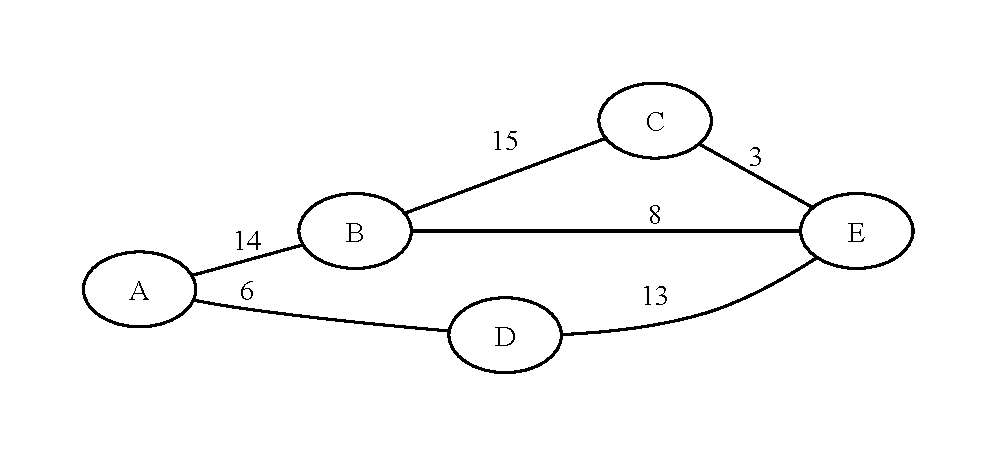
\includegraphics[width = .7\textwidth]{pq_graph.pdf}
\end{center}
Run WhateverFirstSearch(C) using the algorithm below. Initially, all vertices
are unmarked and the bag is empty. The bag is a priority queue: remove the entry
with the smallest priority first. When a neighbor is added, its priority is the
sum of all edge weights along the path used to reach this entry, including the
edge used to add it. The first node added has priority $0$. If bag entries have
the same priority, remove the one with the alphabetically earliest vertex label
first.

\begin{verbatim}
    WhateverFirstSearch(s):
    put s into the bag
    while the bag is not empty:
        take v from the bag
        if v is unmarked:
            mark v
            for each neighbor w of v:
                put w into the bag
\end{verbatim}

In what order are the vertices marked? Write the vertex order below.
\newpage
\item 
What are the strongly connected components in the graph below?
\begin{center}
    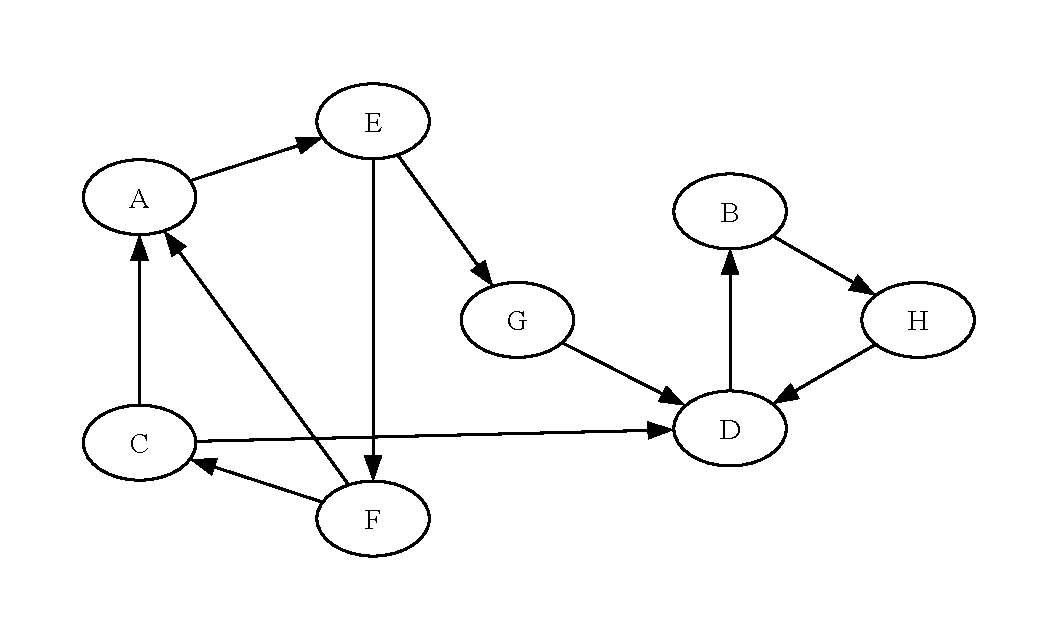
\includegraphics[width=.6\textwidth]{scc_graph.pdf}
\end{center}

\vspace{.5in}

\item
Give the preorder values for all nodes in the following graph. The
$DFS$ and $DFSAll$ algorithms are reproduced below if you need them. Assume
that both process vertices in alphabetical order.
\begin{center}
    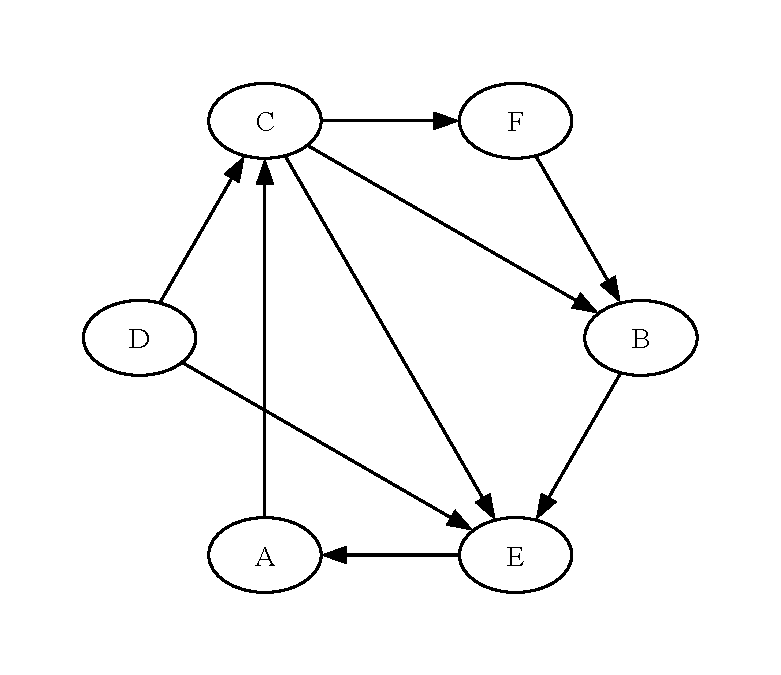
\includegraphics[width=.5\textwidth]{preorder_graph.pdf}
\end{center}

$A.pre = $ \underline{\hspace{.5cm}},
$B.pre = $ \underline{\hspace{.5cm}},
$C.pre = $ \underline{\hspace{.5cm}},
$D.pre = $ \underline{\hspace{.5cm}},
$E.pre = $ \underline{\hspace{.5cm}},
$F.pre = $ \underline{\hspace{.5cm}}

\noindent
\begin{minipage}[t]{0.45\textwidth}
\vspace{0pt}
\small
\begin{verbatim}
DFSAll(G):
  clock = 0
  unmark all vertices
  for each vertex v:
      if v is unmarked:
          clock = DFS(v, clock)
\end{verbatim}
\end{minipage}\hfill
\begin{minipage}[t]{0.45\textwidth}
\vspace{0pt}
\small
\begin{verbatim}
DFS(v, clock):
  mark v
  clock = clock + 1
  v.pre = clock
  for each neighbor w of v:
      if w is unmarked:
          w.parent = v
          clock = DFS(w, clock)
  clock = clock + 1
  v.post = clock
  return clock
\end{verbatim}
\end{minipage}


\end{enumerate}



\end{document}
